\newcommand{\componentA}{0.88}
\newcommand{\componentB}{0.96}
\newcommand{\componentC}{0.997}

\definecolor{motivation}{rgb}{\componentA, \componentB, \componentC}
\definecolor{building}{rgb}{  \componentB, \componentC, \componentA}
\definecolor{basics}{rgb}{    \componentB, \componentA, \componentC}
\definecolor{lists}{rgb}{     \componentA, \componentC, \componentB}
\definecolor{errors}{rgb}{    \componentC, \componentA, \componentB}
\definecolor{templates}{rgb}{ \componentC, \componentB, \componentA}
\definecolor{exercises}{rgb}{ \componentA, \componentB, \componentC}

\newcommand{\bgcolor}{Purple} % this should be renewed below

%%%%%%%%%%%%%%%%%%%%%%%%%%%%%%%%%%%%%%%%%%%%%%%%%%%%%%%%%%%%%%%
%%%%%%%%%%%%%%%%%%%%%%%%%%%%%%%%%%%%%%%%%%%%%%%%%%%% Motivation

% background color pre
{
\setbeamercolor{background canvas}{bg=motivation}
\renewcommand{\bgcolor}{motivation}

\section{Motivation}
\begin{frame}
  \vspace{25mm}
  \begin{center}
    \Huge{Part 1:\\Motivation}
  \end{center}
\end{frame}

\subsection{Observations}
\begin{frame}[fragile]
  \frametitle{Observations}
  \vspace{3mm}
  WYSIWYG editors provide plenty of distractions that compete for your attention.
  \begin{itemize}
    \item That attention is key to good writing.
    \item These distractions slows down the writing process.
  \end{itemize}
  
  \vspace{5mm}
  WYSIWYG editors provide little help managing references of any kind.
  
  \vspace{5mm}
  WYSIWYG editors generally encourage bitmapped graphics.
  
  \vspace{5mm}
  WYSIWYG editors tends to result little consistency in the resulting documents.
  
  \vspace{5mm}
  The formats employed by WISIWYG editors are usually horrible in terms of version control.
  
  \vspace{5mm}
  WISIWYG editors are usually horrible for collaborative editing.
\end{frame}

\subsection{Why \LaTeX?}
\begin{frame}[fragile]
  \frametitle{Why \LaTeX? [1/2]}
  \vspace{3mm}
  \LaTeX\ is a programming language saved in clear text files using markup code.
  \begin{itemize}
    \item This makes it suitable for version control.
    \item Version control is a form of collaborative editing.
    \item Web-based editors (like overleaf) exists and work fairly well.
  \end{itemize}
  
  \vspace{5mm}
  \LaTeX\ (mostly) decouples structure and presentation.
  \begin{itemize}
    \item This results in highly consistent layouts.
    \item When writing, you can focus on the structure.
    \item If you wish to, you can \textsl{choose} to dig into the nitty gritty details.
    \item But there is rarely a need: Most templates make the result look great without intervention.
  \end{itemize}
\end{frame}
\begin{frame}[fragile]
  \frametitle{Why \LaTeX? [2/2]}
  \vspace{2mm}
  \LaTeX\ is a highly extendable and mature system with lots of tools designed for technical documents.
  \begin{itemize}
    \item Working with a bibliography is trivial.
    \item Working with an index is trivial.
    \item Working with floats (like figures and tables) is trivial.
    \item Working with equations is simple.
    \item References to any of these \textsl{just work}.
  \end{itemize}
  
  \vspace{4mm}
  \LaTeX\ is a professional typesetting system and thus vector based.
  \begin{itemize}
    \item It is trivial to include vector graphics.
    \item But it is also trivial to include bitmapped graphics.
  \end{itemize}
  
  \vspace{4mm}
  \textbf{Note:} This essentially mitigates the observations.
\end{frame}

\subsection{What is \LaTeX?}
\begin{frame}[fragile]
  \frametitle{What is \LaTeX?}
  \vspace{3mm}
  \LaTeX\ is a programming language that, when evaluated, produces a PDF file.
  
  \vspace{5mm}
  It relies heavily on the concept of macro expansion.
  
  \vspace{5mm}
  \LaTeX\ is extended through packages. Currently there are 6000+ such packages on CTAN: \url{https://ctan.org}
\end{frame}

\subsection{Styles}
\begin{frame}[fragile]
  \frametitle{What is \LaTeX? \subpart{Styles}}
  \vspace{3mm}
  
\end{frame}

\subsection{When to Not \LaTeX?}
\begin{frame}[fragile]
  \frametitle{When to Not \LaTeX?}
  \vspace{3mm}
  \begin{itemize}
    \descitem{Note Taking} I find that \textsl{markdown} fulfills this role adequately, and is faster to write.
    \descitem{Audience Expectations} Often, your audience will expect a Word file, and then it just doesn't make sense.
  \end{itemize}
\end{frame}

% background color post
}

%%%%%%%%%%%%%%%%%%%%%%%%%%%%%%%%%%%%%%%%%%%%%%%%%%%%%%%%%%%%%%%
%%%%%%%%%%%%%%%%%%%%%%%%%%%%%%%%%%%%%%%%%%%%%% Building the PDF

% background color pre
{
\setbeamercolor{background canvas}{bg=building}
\renewcommand{\bgcolor}{building}

\section{Building the PDF}
\begin{frame}
  \vspace{25mm}
  \begin{center}
    \Huge{Part 2:\\Building the PDF}
  \end{center}
\end{frame}

\subsection{Engines}
\begin{frame}[fragile]
  \frametitle{Engines}
  \vspace{2mm}
  In order to compile a \LaTeX\ document into PDF you need a \LaTeX\ engine.
  
  \vspace{4mm}
  Options:
  \begin{itemize}
    \descitem{pdflatex} The old engine that is fast but lacks native unicode and modern OpenType font support. These are not serious restrictions.
    \descitem{xelatex} A more modern version of \textdesc{pdflatex} that fixes its downsides. But on the flipside it is slower and has not been actively developed since 2017.
    \descitem{lualatex} The most modern engine is scriptable through Lua. It also fixes the issues with \textdesc{pdflatex} and is under active development. It is even slower though.
      \begin{itemize}
        \item This is the way to go for new projects.
        \item From this point on, we will assume \textdesc{lualatex}.
        \item Don't worry too much about the lack of speed. It is rare that it becomes an annoyance.
        \item While you can script it in Lua, the interactions with the \LaTeX\ macro system are complex. Personally, I have decided against it.
      \end{itemize}
  \end{itemize}
\end{frame}

\subsection{Distributions}
\begin{frame}[fragile]
  \frametitle{Distributions}
  \vspace{3mm}
  For you to work with \LaTeX, you will need:
  \begin{itemize}
    \item A number of appropriate fonts.
    \item A \LaTeX\ engine for compiling.
    \item A collection of packages with extensions.
    \item A number of other support programs.
  \end{itemize}
  
  \vspace{5mm}
  All of this combined is referred to as a \LaTeX\ distribution.
  
  \vspace{5mm}
  There exists a number of precompiled distributions:
  \begin{itemize}
    \descitem{\TeX\ Live} The typical distribution (Linux, Windows and OSX).
    \descitem{MiKTeX} If you are on Windows (but also works in Linux and OSX).
    \descitem{MacTeX} If you are on a Mac.
  \end{itemize}
\end{frame}

\subsection{Commandline}
\begin{frame}[fragile]
  \frametitle{Commandline}
  \vspace{3mm}
  Running the \LaTeX\ interpreter is done using the following command:
  \begin{minted}[breaklines]{shell-session}
lualatex document.tex
  \end{minted}
  or, if you are using \packagename{minted} for source code highlighting:
  \begin{minted}[breaklines]{shell-session}
lualatex -shell-escape document.tex
  \end{minted}
  
  \vspace{5mm}
  \textbf{Note:} When using references, you may have to run the command multiple times.
\end{frame}

\subsection{Overleaf}
\begin{frame}[fragile]
  \frametitle{Overleaf}
  \begin{tikzpicture}[remember picture,overlay]
    \node[anchor=south] () at ([yshift=-1.2cm]current page.south) {
      \only<1>{\includeBitmap{overleafmain.png}{14cm}}\only<2>{\includeBitmap{overleafdemo.png}{14cm}}
    };
  \end{tikzpicture}
\end{frame}

\subsubsection{Hosting Options}
\begin{frame}[fragile]
  \frametitle{Overleaf \subpart{Hosting Options}}
  \vspace{3mm}
  Cloud:
  \begin{itemize}
    \item Paid and free tier.
    \item Paid tier provices GIT support.
    \item Issues with uptime.
  \end{itemize}
  
  \vspace{5mm}
  Self-hosted:
  \begin{itemize}
    \item No GIT support.
    \item If all else fails, you can pull the data out yourself.
  \end{itemize}
\end{frame}

\subsection{Make}
\begin{frame}[fragile]
  \frametitle{Make}
  \vspace{-1mm}
  \inputminted[fontsize=\tiny]{make}{Makefile}
\end{frame}

\subsection{GIT}
\begin{frame}[fragile]
  \frametitle{GIT}
  \vspace{3mm}
  GIT is used for keeping tract of revisions of (primarily) human-readable files.
  
  \vspace{5mm}
  This is usually used for program code.
  
  \vspace{5mm}
  \LaTeX\ is a programming language, and when we execute \LaTeX\ code (through an interpreter) then we get a PDF file.
  
  \vspace{5mm}
  A GIT repository can easily contain both your program code and your report.
  
  \vspace{5mm}
  Typical structure:
  \begin{itemize}
    \item Program code in \textcolor{purple}{\texttt{/src}} of the repository.
    \item Report and presentation in \textcolor{purple}{\texttt{/doc}} of the repository.
    \item Figures shared between report an presentation in \textcolor{purple}{\texttt{/doc/figs}} of the repository.
  \end{itemize}
\end{frame}

% background color post
}

%%%%%%%%%%%%%%%%%%%%%%%%%%%%%%%%%%%%%%%%%%%%%%%%%%%%%%%%%%%%%%%
%%%%%%%%%%%%%%%%%%%%%%%%%%%%%%%%%%%%%%%%%%%%%%%%%%%%%%%% Basics

% background color pre
{
\setbeamercolor{background canvas}{bg=basics}
\renewcommand{\bgcolor}{basics}

\section{Basics}
\begin{frame}
  \vspace{25mm}
  \begin{center}
    \Huge{Part 3:\\Basics}
  \end{center}
\end{frame}

\subsection{Overall Structure}
\begin{frame}[fragile]
  \frametitle{Overall Structure}
  \begin{tikzpicture}[remember picture,overlay]
    \newcommand{\height}[0]{14mm}
    \newcommand{\width}[0]{3mm}
    
    \tikzstyle{segment} = [
      rectangle,
      rounded corners=1mm,
      anchor=north west,
      fill=purple,
      minimum height=\height,
      minimum width=\width,
    ]
    
    \coordinate (top) at ([yshift=34mm]current page.center);
    
    \node[anchor=north] (docclass) at (top) {\mintinline{latex}{\documentclass[a4paper, oneside]{memoir}}};
    
    \node[segment] (pa) at (docclass.south west) {};
    \node[anchor=west] () at (pa.east) {Preample};
    
    \node[anchor=north west] (begin) at (pa.south west) {\mintinline{latex}{\begin{document}}};
    
    \node[segment] (fm) at (begin.south west) {};
    \node[anchor=west] () at (fm.east) {Front Matter};
    
    \node[segment] (main) at (fm.south west) {};
    \node[anchor=west] () at (main.east) {Main Matter};
    
    \node[segment] (bm) at (main.south west) {};
    \node[anchor=west] () at (bm.east) {Back Matter};
    
    \node[anchor=north west] (end) at (bm.south west) {\mintinline{latex}{\end{document}}};
  \end{tikzpicture}
\end{frame}

\subsection{Packages}
\begin{frame}[fragile]
  \frametitle{Packages}
  \vspace{3mm}
  
\end{frame}

\subsection{Language and Hyphenation}
\begin{frame}[fragile]
  \frametitle{Language and Hyphenation}
  \vspace{3mm}
  
\end{frame}

\subsubsection{Document Parts}
\begin{frame}[fragile]
  \frametitle{Overall Structure \subpart{Document Parts}}
  \vspace{3mm}
  
\end{frame}

\subsubsection{File Inclusion}
\begin{frame}[fragile]
  \frametitle{Overall Structure \subpart{File Inclusion}}
  \vspace{3mm}
  
\end{frame}

\subsubsection{Sectioning}
\begin{frame}[fragile]
  \frametitle{Overall Structure \subpart{Sectioning}}
  \vspace{3mm}
  
\end{frame}

\subsection{Spacing}
\begin{frame}[fragile]
  \frametitle{Spacing}
  \vspace{3mm}
  Whitespaces are treated the same way as in most other programming languages: Either there is at least one, or there is none. No need to worry about having two spaces instead of one.
  
  \vspace{5mm}
  Horizontal and vertical space can be added with the \commandname{hspace} and \commandname{vspace} commands. They both take one parameter; a distance.
  
  \vspace{5mm}
  \LaTeX\ will break the line as it tries to optimize the document layout (by minimizing \textsl{badness}) according to the rules of the style.
  
  \vspace{5mm}
  \textbf{Note:} This can make it hard to force a specific placement.
\end{frame}

\subsubsection{Horizontal Space}
\begin{frame}[fragile]
  \frametitle{Spacing \subpart{Horizontal Space}}
  \vspace{3mm}
  \begin{tikzpicture}[remember picture,overlay]
    \newcommand{\height}[0]{24mm}
    \newcommand{\dist}[0]{5mm}
    
    \tikzstyle{dedge} = [thick,->,>=stealth,draw=black]
    
    \node[rectangle,thick,anchor=east,draw,minimum height=\height] (code) at ([xshift=-\dist]current page.center) {
      \begin{minipage}{6cm}
        \begin{minted}[breaklines]{latex}
first\hspace{1cm}last
        \end{minted}
      \end{minipage}
    };
    
    \node[rectangle,thick,anchor=west,draw,minimum height=\height] (output) at ([xshift=\dist]current page.center) {
      \begin{minipage}{6cm}
        first\hspace{1cm}last
      \end{minipage}
    };
    
    \draw[dedge] (code)->(output);
  \end{tikzpicture}
\end{frame}

\subsubsection{Vertical Space}
\begin{frame}[fragile]
  \frametitle{Spacing \subpart{Vertical Space}}
  \vspace{3mm}
  \begin{tikzpicture}[remember picture,overlay]
    \newcommand{\height}[0]{24mm}
    \newcommand{\dist}[0]{5mm}
    
    \tikzstyle{dedge} = [thick,->,>=stealth,draw=black]
    
    \node[rectangle,thick,anchor=east,draw,minimum height=\height] (code) at ([xshift=-\dist]current page.center) {
      \begin{minipage}{6cm}
        \begin{minted}[breaklines]{latex}
first

\vspace{1cm}
last
        \end{minted}
      \end{minipage}
    };
    
    \node[rectangle,thick,anchor=west,draw,minimum height=\height] (output) at ([xshift=\dist]current page.center) {
      \begin{minipage}{6cm}
        first
        
        \vspace{1cm}
        last
      \end{minipage}
    };
    
    \draw[dedge] (code)->(output);
  \end{tikzpicture}
\end{frame}

\subsection{Formatting}
\begin{frame}[fragile]
  \frametitle{Formatting}
  \vspace{18mm}
  
  \begin{tikzpicture}[remember picture,overlay]
    \newcommand{\height}[0]{36mm}
    \newcommand{\dist}[0]{5mm}
    
    \tikzstyle{dedge} = [thick,->,>=stealth,draw=black]
    
    \node[rectangle,thick,anchor=east,draw,minimum height=\height] (code) at ([xshift=-\dist]current page.center) {
      \begin{minipage}{5cm}
        \begin{minted}{latex}
normal \\
\textbf{bold} \\
\textsl{slanted} \\
\textit{italics} \\
\texttt{teletype} \\
\textsl{serif free} \\
\underline{underline}
        \end{minted}
      \end{minipage}
    };
    
    \node[rectangle,thick,anchor=west,draw,minimum height=\height] (output) at ([xshift=\dist]current page.center) {
      \begin{minipage}{5cm}
        normal \\
        \textbf{bold} \\
        \textsl{slanted} \\
        \textit{italics} \\
        \texttt{teletype} \\
        \textsl{serif free} \\
        \underline{underline}
      \end{minipage}
    };
    
    \draw[dedge] (code)->(output);
  \end{tikzpicture}
\end{frame}

\subsection{Text Size}
\begin{frame}[fragile]
  \frametitle{Text Size}
  \vspace{8mm}
  
  \begin{tikzpicture}[remember picture,overlay]
    \newcommand{\height}[0]{50mm}
    \newcommand{\dist}[0]{5mm}
    
    \tikzstyle{dedge} = [thick,->,>=stealth,draw=black]
    
    \node[rectangle,thick,anchor=east,draw,minimum height=\height] (code) at ([xshift=-\dist]current page.center) {
      \begin{minipage}{6cm}
        \begin{minted}[breaklines]{latex}
\tiny{Sample text}
\scriptsize{Sample text}
\footnotesize{Sample text}
\small{Sample text}
\normalsize{Sample text}
\large{Sample text}
\Large{Sample text}
\LARGE{Sample text}
\huge{Sample text}
\Huge{Sample text}
        \end{minted}
      \end{minipage}
    };
    
    \node[rectangle,thick,anchor=west,draw,minimum height=\height] (output) at ([xshift=\dist]current page.center) {
      \begin{minipage}{6cm}
        \tiny{Sample text}
        \scriptsize{Sample text}
        \footnotesize{Sample text}
        \small{Sample text}
        \normalsize{Sample text}
        \large{Sample text}
        \Large{Sample text}
        \LARGE{Sample text}
        \huge{Sample text}
        \Huge{Sample text}
      \end{minipage}
    };
    
    \draw[dedge] (code)->(output);
  \end{tikzpicture}
\end{frame}

\subsection{Listings}
\begin{frame}[fragile]
  \frametitle{Listings}
  \vspace{3mm}
  General considerations when deciding between ordered or unordered lists:
  
  \begin{tikzpicture}[remember picture,overlay]
    \newcommand{\dist}[0]{10mm}
    \newcommand{\decision}[1]{\textsl{#1}}
    
    \tikzstyle{choice} = [
      diamond,
      thick,
      draw=black,
      align=center,
      inner sep=0pt,
    ]
    \tikzstyle{outcome} = [
      rectangle,
      thick,
      draw=black,
      anchor=north,
      align=center,
      minimum width=4.85cm,
      minimum height=8mm,
    ]
    
    \tikzstyle{dedge} = [thick,->,>=stealth,draw=black]
    
    \node[matrix,column sep=\dist,row sep=\dist] () at ([yshift=-1cm]current page.center) {
      &
      &
      &
      \node[outcome,anchor=west] (enumerate) {use \commandname{enumerate} environment};
      \\
      \node[] (origin) {};
      &
      \node[choice,anchor=east] (choiceA) {mentioned\\the number\\of items?};
      &
      \node[choice] (choiceB) {need to\\refer to a\\specific\\item?};
      &
      \node[outcome,anchor=west] (itemize) {use \commandname{itemize} environment};
      \\
    };
    
    \node[anchor=east] () at ([yshift=\dist/2]choiceA.north) {\decision{yes}};
    \node[anchor=east] () at ([yshift=\dist/2]choiceB.north) {\decision{yes}};
    
    \draw[dedge] (origin)--(choiceA);
    \draw[dedge] (choiceA)--(choiceB) node[midway,sloped,below] {\decision{no}};
    \draw[dedge] (choiceB)--(itemize) node[midway,sloped,below] {\decision{no}};
    \draw[dedge] (choiceA)|-([yshift= 2mm]enumerate.west);
    \draw[dedge] (choiceB)|-([yshift=-2mm]enumerate.west);
  \end{tikzpicture}
\end{frame}

\subsubsection{Itemization}
\begin{frame}[fragile]
  \frametitle{Listings \subpart{Itemization}}
  \vspace{18mm}
  
  \begin{tikzpicture}[remember picture,overlay]
    \newcommand{\height}[0]{36mm}
    \newcommand{\dist}[0]{5mm}
    
    \tikzstyle{dedge} = [thick,->,>=stealth,draw=black]
    
    \node[rectangle,thick,anchor=east,draw,minimum height=\height] (code) at ([xshift=-\dist]current page.center) {
      \begin{minipage}{5cm}
        \begin{minted}{latex}
Programming languages:
\begin{itemize}
  \item Rust
  \item Elixir
  \item Python
  \item \LaTeX ?
\end{itemize}
        \end{minted}
      \end{minipage}
    };
    
    \node[rectangle,thick,anchor=west,draw,minimum height=\height] (output) at ([xshift=\dist]current page.center) {
      \begin{minipage}{5cm}
        Programming languages:
        \begin{itemize}
          \item Rust
          \item Elixir
          \item Python
          \item \LaTeX ?
        \end{itemize}
      \end{minipage}
    };
    
    \draw[dedge] (code)->(output);
  \end{tikzpicture}
\end{frame}

\subsubsection{Enumerations}
\begin{frame}[fragile]
  \frametitle{Listings \subpart{Enumerations}}
  \vspace{18mm}
  
  \begin{tikzpicture}[remember picture,overlay]
    \newcommand{\height}[0]{36mm}
    \newcommand{\dist}[0]{5mm}
    
    \tikzstyle{dedge} = [thick,->,>=stealth,draw=black]
    
    \node[rectangle,thick,anchor=east,draw,minimum height=\height] (code) at ([xshift=-\dist]current page.center) {
      \begin{minipage}{5cm}
        \begin{minted}{latex}
Programming languages:
\begin{enumerate}
  \item Rust
  \item Elixir
  \item Python
  \item \LaTeX ?
\end{enumerate}
        \end{minted}
      \end{minipage}
    };
    
    \node[rectangle,thick,anchor=west,draw,minimum height=\height] (output) at ([xshift=\dist]current page.center) {
      \begin{minipage}{5cm}
        Programming languages:
        \begin{enumerate}
          \item Rust
          \item Elixir
          \item Python
          \item \LaTeX ?
        \end{enumerate}
      \end{minipage}
    };
    
    \draw[dedge] (code)->(output);
  \end{tikzpicture}
\end{frame}

\subsection{References}
\begin{frame}[fragile]
  \frametitle{References}
  \vspace{3mm}
  Numbered \textsl{things} can be labeled and referenced by their number or their page.
  
  \vspace{5mm}
  These include:
  \begin{itemize}
    \item Section at any level of depth.
    \item Figures and tables.
    \item Equations.
    \item Enumerated lists.
  \end{itemize}
  
  \vspace{5mm}
  They do not include:
  \begin{itemize}
    \item Bibliography.
  \end{itemize}
\end{frame}

\subsubsection{Use}
\begin{frame}[fragile]
  \frametitle{References \subpart{Use}}
  \vspace{3mm}
  A label is created using the \commandname{label} command. This will refer to the latest numerable construct.
  
  \vspace{5mm}
  The number referred to by a label can be accessed using the \commandname{ref} command. Be sure to preface it with something that indicates what you are referring to (e.g., a section).
  
  \vspace{5mm}
  The page number containing a label can be accessed using the \commandname{pageref} command.
  
  \vspace{5mm}
  \textbf{Note:} References need two parses of the \LaTeX\ compiler to function:
  \begin{itemize}
    \item First pass notes down the position of the labels.
    \item Second pass inserts these positions at the references.
  \end{itemize}
\end{frame}

\subsubsection{Example}
\begin{frame}[fragile]
  \frametitle{References \subpart{Example}}
  \begin{tikzpicture}[remember picture,overlay]
    \newcommand{\height}[0]{32mm}
    \newcommand{\dist}[0]{5mm}
    
    \tikzstyle{dedge} = [thick,->,>=stealth,draw=black]
    
    \node[rectangle,thick,anchor=east,draw,minimum height=\height] (code) at ([xshift=-\dist]current page.center) {
      \begin{minipage}{6cm}
        \begin{minted}{latex}
Algorithm:
\begin{enumerate}
  \item Initialize.
  \item \label{id} Do stuff.
  \item Go to \ref{id}.
\end{enumerate}
        \end{minted}
      \end{minipage}
    };
    
    \node[rectangle,thick,anchor=west,draw,minimum height=\height] (output) at ([xshift=\dist]current page.center) {
      \begin{minipage}{6cm}
        Algorithm:
        \begin{enumerate}
          \item Initialize.
          \item \label{id} Do stuff.
          \item Go to step \ref{id}.
        \end{enumerate}
      \end{minipage}
    };
    
    \draw[dedge] (code)->(output);
  \end{tikzpicture}
\end{frame}

\subsection{Colors}
\begin{frame}[fragile]
  \frametitle{Colors}
  \vspace{3mm}
  \LaTeX\ provides a set of predefined color names: \url{https://latexcolor.com}
\end{frame}

\subsection{Predefined}
\begin{frame}[fragile]
  \frametitle{Colors \subpart{Predefined}}
  \begin{tikzpicture}[remember picture,overlay]
    \node[anchor=south] () at ([yshift=-1cm]current page.south) {
      \includeBitmap{latexcolor.png}{14cm}
    };
  \end{tikzpicture}
\end{frame}

\subsection{Tables}
\begin{frame}[fragile]
  \frametitle{Tables}
  \vspace{3mm}
  
\end{frame}

\subsection{Including Visuals}
\begin{frame}[fragile]
  \frametitle{Including Visuals}
  \vspace{3mm}
  When it comes to visual aids, \LaTeX\ supports a number of different types.
  
  \begin{center}
    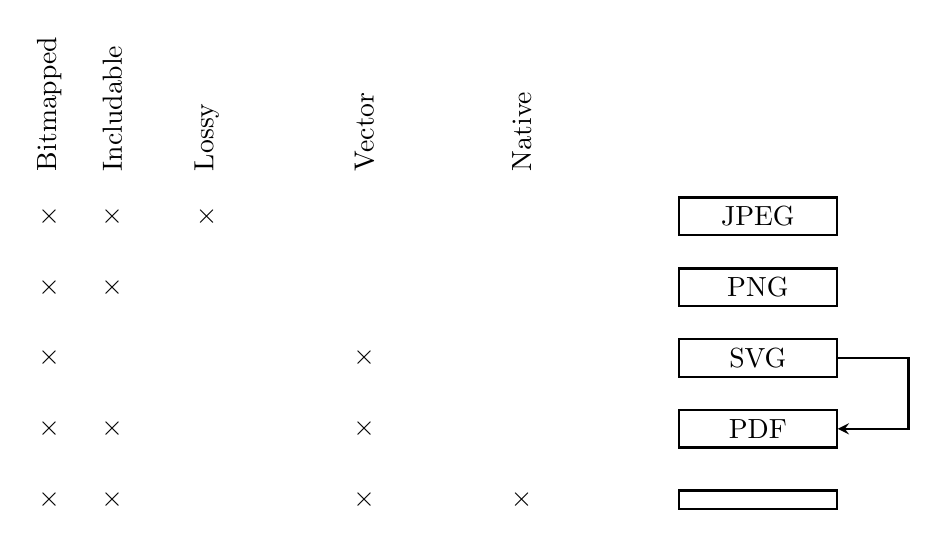
\begin{tikzpicture}[]
      \newcommand{\bitmapX}[0]{0mm}
      \newcommand{\lossyX}[0]{20mm}
      \newcommand{\vectorX}[0]{40mm}
      \newcommand{\stylableX}[0]{60mm}
      \newcommand{\includableX}[0]{8mm}
      \newcommand{\formatX}[0]{90mm}
      \newcommand{\convertX}[0]{120mm}
      
      \newcommand{\stepY}[0]{-9mm}
      
      \tikzstyle{label} = []
      \tikzstyle{format} = [
        rectangle,
        thick,
        draw,
        minimum width=2cm,
      ]
      
      \tikzstyle{dedge} = [thick,->,>=stealth,draw=black]
      
      \node[label,anchor=south] () at (\bitmapX, -0.5*\stepY) {\rotatebox{90}{Bitmapped}};
      \node[label,anchor=south] () at (\lossyX, -0.5*\stepY) {\rotatebox{90}{Lossy}};
      \node[label,anchor=south] () at (\vectorX, -0.5*\stepY) {\rotatebox{90}{Vector}};
      \node[label,anchor=south] () at (\stylableX, -0.5*\stepY) {\rotatebox{90}{Native}};
      \node[label,anchor=south] () at (\includableX, -0.5*\stepY) {\rotatebox{90}{Includable}};
      
      \node[label] () at (\bitmapX, 0*\stepY) {$\times$};
      \node[label] () at (\lossyX, 0*\stepY) {$\times$};
      \node[label] () at (\includableX, 0*\stepY) {$\times$};
      \node[format] () at (\formatX, 0*\stepY) {JPEG};
      
      \node[label] () at (\bitmapX, 1*\stepY) {$\times$};
      \node[label] () at (\includableX, 1*\stepY) {$\times$};
      \node[format] () at (\formatX, 1*\stepY) {PNG};
      
      \node[label] () at (\bitmapX, 2*\stepY) {$\times$};
      \node[label] () at (\vectorX, 2*\stepY) {$\times$};
      \node[format] (svg) at (\formatX, 2*\stepY) {SVG};
      
      \node[label] () at (\bitmapX, 3*\stepY) {$\times$};
      \node[label] () at (\vectorX, 3*\stepY) {$\times$};
      \node[label] () at (\includableX, 3*\stepY) {$\times$};
      \node[format] (pdf) at (\formatX, 3*\stepY) {PDF};
      
      \node[label] () at (\bitmapX, 4*\stepY) {$\times$};
      \node[label] () at (\vectorX, 4*\stepY) {$\times$};
      \node[label] () at (\stylableX, 4*\stepY) {$\times$};
      \node[label] () at (\includableX, 4*\stepY) {$\times$};
      \node[format] () at (\formatX, 4*\stepY) {\TikZ};
      
      \draw[dedge] (svg)
                 --([xshift=-\stepY]svg.east)
                 --([xshift=-\stepY]pdf.east)
                 --(pdf);
    \end{tikzpicture}
  \end{center}
\end{frame}

\subsubsection{PDF Graphics}
\begin{frame}[fragile]
  \frametitle{Including Visuals \subpart{PDF Graphics}}
  \vspace{3mm}
  
\end{frame}

\subsubsection{SVG Graphics}
\begin{frame}[fragile]
  \frametitle{Including Visuals \subpart{SVG Graphics}}
  \vspace{3mm}
  
\end{frame}

\subsubsection{Bitmapped Graphics}
\begin{frame}[fragile]
  \frametitle{Including Visuals \subpart{Bitmapped Graphics}}
  \vspace{3mm}
  
\end{frame}

\subsection{Figures}
\begin{frame}[fragile]
  \frametitle{Figures}
  \vspace{3mm}
  
\end{frame}

\subsection{Footnotes}
\begin{frame}[fragile]
  \frametitle{Footnotes}
  \begin{tikzpicture}[remember picture,overlay]
    \newcommand{\height}[0]{24mm}
    \newcommand{\dist}[0]{5mm}
    
    \tikzstyle{dedge} = [thick,->,>=stealth,draw=black]
    
    \node[rectangle,thick,anchor=east,draw,minimum height=\height] (code) at ([xshift=-\dist]current page.center) {
      \begin{minipage}{6cm}
        \begin{minted}{latex}
Text\footnote{Short
detaining.}.
        \end{minted}
      \end{minipage}
    };
    
    \node[rectangle,thick,anchor=west,draw,minimum height=\height] (output) at ([xshift=\dist]current page.center) {
      \begin{minipage}{6cm}
        Text\footnote{Short
        detaining.}.
      \end{minipage}
    };
    
    \draw[dedge] (code)->(output);
  \end{tikzpicture}
\end{frame}

\subsection{Margin Paragraphs}
\begin{frame}[fragile]
  \frametitle{Margin Paragraphs}
  \vspace{3mm}
  Margin paragraphs works in much the same way as footnotes.
  
  \vspace{5mm}
  However, they are (i) not numbered, and (ii) appear in the outer margin.
  
  \vspace{5mm}
  Instead of the \commandname{footnote} command you use \commandname{marginpar} (and make sure that the \packagename{marginnote} package is included).
  
  \begin{tikzpicture}[remember picture,overlay]
    \node[anchor=south] () at ([yshift=-42mm]current page.south) {
      \includeBitmap{marginpar.png}{14cm}
    };
  \end{tikzpicture}
\end{frame}

\subsection{Code Inclusion}
\begin{frame}[fragile]
  \frametitle{Code Inclusion}
  \vspace{3mm}
  There is a number of packages for including code. In this presentation we will look at \packagename{minted}.
  
\end{frame}

\subsection{Mathematics}
\begin{frame}[fragile]
  \frametitle{Mathematics}
  \vspace{3mm}
  
\end{frame}

\subsubsection{Inline}
\begin{frame}[fragile]
  \frametitle{Mathematics \subpart{Inline}}
  \begin{tikzpicture}[remember picture,overlay]
    \newcommand{\height}[0]{24mm}
    \newcommand{\dist}[0]{5mm}
    
    \tikzstyle{dedge} = [thick,->,>=stealth,draw=black]
    
    \node[rectangle,thick,anchor=east,draw,minimum height=\height] (code) at ([xshift=-\dist]current page.center) {
      \begin{minipage}{6cm}
        \begin{minted}{latex}
The Pythagorean theorem
states that $a^2+b^2 = c^2$,
but can also be expressed as
$c = \sqrt{a^2+b^2}$.
        \end{minted}
      \end{minipage}
    };
    
    \node[rectangle,thick,anchor=west,draw,minimum height=\height] (output) at ([xshift=\dist]current page.center) {
      \begin{minipage}{6cm}
        The Pythagorean theorem states that $a^2+b^2 = c^2$, but can also be expressed as $c = \sqrt{a^2+b^2}$.
      \end{minipage}
    };
    
    \draw[dedge] (code)->(output);
  \end{tikzpicture}
\end{frame}

\subsubsection{Equations}
\begin{frame}[fragile]
  \frametitle{Mathematics \subpart{Equations}}
  \vspace{3mm}
  
\end{frame}

\subsubsection{Equation References}
\begin{frame}[fragile]
  \frametitle{Mathematics \subpart{Equation References}}
  \vspace{3mm}
  
\end{frame}

\subsection{URLs}
\begin{frame}[fragile]
  \frametitle{URLs}
  \vspace{3mm}
  \begin{tikzpicture}[remember picture,overlay]
    \newcommand{\height}[0]{36mm}
    \newcommand{\dist}[0]{5mm}
    
    \tikzstyle{dedge} = [thick,->,>=stealth,draw=black]
    
    \node[rectangle,thick,anchor=east,draw,minimum height=\height] (code) at ([xshift=-\dist]current page.center) {
      \begin{minipage}{6cm}
        \begin{minted}[fontsize=\scriptsize]{latex}
Search at
\textcolor{blue}{
  \texttt{https://search.brave.com}
}

Search at
\url{https://search.brave.com}

Search at
\href{https://search.brave.com}{Brave}
        \end{minted}
      \end{minipage}
    };
    
    \node[rectangle,thick,anchor=west,draw,minimum height=\height] (output) at ([xshift=\dist]current page.center) {
      \scriptsize
      \begin{minipage}{6cm}
Search at
\textcolor{blue}{https://search.brave.com}

\vspace{3mm}
Search at
\url{https://search.brave.com}

\vspace{3mm}
Search at
\href{https://search.brave.com}{Brave}
      \end{minipage}
    };
    
    \draw[dedge] (code)->(output);
  \end{tikzpicture}
\end{frame}

\subsection{Nooks and Crannies}
\begin{frame}[fragile]
  \frametitle{Nooks and Crannies}
  \vspace{3mm}
  The \commandname{\textbackslash ldots} can be used to add three periods \ldots
  
  \vspace{5mm}
  Just as the \commandname{\textbackslash LaTeX} command, it will eat any following space. If this is not what you want, then you have to escape the following space with a backslash.
\end{frame}

% background color post
}

%%%%%%%%%%%%%%%%%%%%%%%%%%%%%%%%%%%%%%%%%%%%%%%%%%%%%%%%%%%%%%%
%%%%%%%%%%%%%%%%%%%%%%%%%%%%%%%%%%%%%%%%%%%%%%%%%%%%%%%%% Lists

% background color pre
{
\setbeamercolor{background canvas}{bg=lists}
\renewcommand{\bgcolor}{lists}

\section{Lists}
\begin{frame}
  \vspace{25mm}
  \begin{center}
    \Huge{Part 4:\\Lists}
  \end{center}
\end{frame}

\subsection{Table of Contents}
\begin{frame}[fragile]
  \frametitle{Table of Contents}
  \vspace{3mm}
  
\end{frame}

\subsection{List of Figures}
\begin{frame}[fragile]
  \frametitle{List of Figures}
  \vspace{3mm}
  
\end{frame}

\subsection{List of Tables}
\begin{frame}[fragile]
  \frametitle{List of Tables}
  \vspace{3mm}
  
\end{frame}

\subsection{Bibliography}
\begin{frame}[fragile]
  \frametitle{Bibliography}
  \vspace{3mm}
  
\end{frame}

\subsection{Index}
\begin{frame}[fragile]
  \frametitle{Index}
  \vspace{3mm}
  
\end{frame}

% background color post
}

%%%%%%%%%%%%%%%%%%%%%%%%%%%%%%%%%%%%%%%%%%%%%%%%%%%%%%%%%%%%%%%
%%%%%%%%%%%%%%%%%%%%%%%%%%%%%%%%%%%%%%%%%%% Dealing with Errors

% background color pre
{
\setbeamercolor{background canvas}{bg=errors}
\renewcommand{\bgcolor}{errors}

\section{Dealing with Errors}
\begin{frame}
  \vspace{25mm}
  \begin{center}
    \Huge{Part 5:\\Dealing with Errors}
  \end{center}
\end{frame}

\subsection{Locating the Error}
\begin{frame}[fragile]
  \frametitle{Locating the Error}
  \vspace{3mm}
  
\end{frame}

\subsection{Googling the Error}
\begin{frame}[fragile]
  \frametitle{Googling the Error}
  \vspace{3mm}
  
\end{frame}

% background color post
}

%%%%%%%%%%%%%%%%%%%%%%%%%%%%%%%%%%%%%%%%%%%%%%%%%%%%%%%%%%%%%%%
%%%%%%%%%%%%%%%%%%%%%%%%%%%%%%%%%%%%%%%%%%%%%%%%%%%%% Templates

% background color pre
{
\setbeamercolor{background canvas}{bg=templates}
\renewcommand{\bgcolor}{templates}

\section{Templates}
\begin{frame}
  \vspace{25mm}
  \begin{center}
    \Huge{Part 6:\\Templates}
  \end{center}
\end{frame}

\subsection{Source}
\begin{frame}[fragile]
  \frametitle{Source}
  \vspace{3mm}
  The source code for these slides can be found here: \url{https://github.com/aslakjohansen/prosa-latex}
\end{frame}

\subsection{Reports}
\begin{frame}[fragile]
  \frametitle{Reports}
  \vspace{3mm}
  
\end{frame}

\subsection{Presentations}
\begin{frame}[fragile]
  \frametitle{Presentations}
  \vspace{3mm}
  
\end{frame}

% background color post
}

%%%%%%%%%%%%%%%%%%%%%%%%%%%%%%%%%%%%%%%%%%%%%%%%%%%%%%%%%%%%%%%
%%%%%%%%%%%%%%%%%%%%%%%%%%%%%%%%%%%%%%%%%%%%%%%%%%%%% Exercises

% background color pre
{
\setbeamercolor{background canvas}{bg=exercises}
\renewcommand{\bgcolor}{exercises}

\section{Exercises}
\begin{frame}
  \vspace{25mm}
  \begin{center}
    \Huge{Part 7:\\Exercises}
  \end{center}
\end{frame}

\subsection{Exercises}
\begin{frame}[fragile]
  \frametitle{Exercises}
  \vspace{3mm}
  \begin{enumerate}
    \descitem{New Project:} Create a new project (on Overleaf, GitHub or similar). Make sure that you have a report \LaTeX\ document that builds.
    \descitem{Tabular Data:} Find some tabular data, place it in a \texttt{tabular} environment, and make it look pretty.
    \descitem{Report:} Pick any old report, and port it to \LaTeX. The point is not to go through the whole report, but rather to get a feel of (i) the effort needed to port an old report, and (ii) the perceived typographical quality per effort.
  \end{enumerate}
\end{frame}

% background color post
}

